\documentclass[a4paper,10pt,twocolumn,dvipdfmx]{jsarticle}
\usepackage[dvipdfmx]{graphicx}
\usepackage{tikz}
\usepackage{here}
\usepackage{array,booktabs}
\usetikzlibrary{patterns}

\title{二次元重複面積直接計算による高速並進運動粉粒体の\\
自己相関関数と並進運動粉粒体の仮現運動速度の比較(仮)
%Comparative evaluation of autocorrelation function of time-dependent configuration of particulate/powdery systems in fast translational motion and the velocity of the apparent motion of them
}
\author{吉渡 匠汰}
\date{ } %change

%\setlength{\textwidth}{155truemm}
%\setlength{\fullwidth}{\textwidth}
%\setlength{\oddsidemargin}{37truemm}
%\addtolength{\oddsidemargin}{-1truein}
%\setlength{\topmargin}{30truemm}
%\setlength{\textheight}{237truemm}
%\addtolength{\topmargin}{-1truein}

\begin{document}
\twocolumn[
\maketitle
\begin{abstract}
工場ではモニターを用いて粉体を観察しているが、その作業は目視によるものである。しかし、目視で異常を判断するのは難しいことである。よって筆者らは画像処理を用いた粉体の運動の測定を行った。 \par
\end{abstract}
] 

\section{序章}
工場ではモニターを用いて粉体を観察しているが、その作業は目視によるものである。しかし、目視で異常を判断するのは難しいことである。よって筆者らは画像処理を用いた粉体の運動の測定を行った。
\section{物体の運動評価法}
我々が落下している物体を見て、それが球であるか液体であるかを判断する要因としては相関の崩れが考えられる。すなわち落下運動を見始めたときと、その一瞬後の光景がどれだけ異なっているかということである。また、見始めたときの光景をいつまでも記憶しているわけではないからこの比較は短時間でリセットされ、今の状態を記憶、一瞬後との比較が繰り返されているものと思われる。
\subsection{相関関数の評価方法}
相関つまり初期状態からの物体の相関を次のように定義する。$「物体の初期状態(t=t)と現在の状態(t=t+\Delta t)の重なり」$である。例として1つの球が落下する場合を考える。落下しているある時点を初期状態とし、その数ミリ秒後には球が半径分移動したとする(図\ref{fig:exfall}左)。このとき、2つの球の重なりは図\ref{fig:exfall}の左斜線部分である。この後重なり面積は徐々に小さくなっていき、球1つ分移動した後には完全に重なりは0となる。
また、しばらく経過すると異なる物体が重なることになるが、この場合の重なりも計算している(\ref{fig:exfall}の右)。もし、同一物体の重なりが完全に外れても高い相関を示し続けた場合、落下パターンがほぼ一定であることを示している。
\begin{figure}[hbtp]
\centering
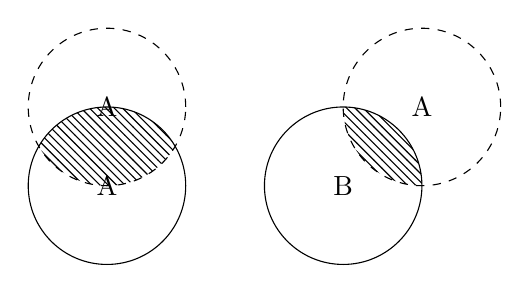
\begin{tikzpicture}
%左
\begin{scope}
\node (A0) at (0,0) {A};
\node (A) at (0,1) {A};
\clip (0,0) circle (1);
\fill[black, thick, pattern=north west lines] (0,1) circle(1);
\end{scope}
\node (A0) at (3,0) {B};
\node (A) at (4,1) {A};
\draw (0,0) circle(1);
\draw [dashed](0,1) circle(1);
%右
\begin{scope}
\clip (3,0) circle (1);
\fill[black, thick, pattern=north west lines] (4,1) circle(1);
\end{scope}
\draw (3,0) circle(1);
\draw [dashed](4,1) circle(1);
\end{tikzpicture}
\caption{落下運動の例 破線は比較される初期座標}
\label{fig:exfall}
\end{figure}
\subsection{画像処理について}
物体の重なりの相関をとるため、物体がどこにあるかを正確に検出する必要がある。そのために本研究では二値化という手法を用いている。二値化とは各画素について一定の閾値ならば白、そうでないならば黒にするという処理を施し、白黒の画像を作成する処理である。運動する対象の色とギャップの大きい色を背景にして撮影し、二値化処理によって対象を白または黒で抜き出すことができる。 \par
二値化処理を施した画像の例として図\ref{fig:threshold}を示す。
初期状態での二値化画像と別なタイミングの二値化画像を重ね、白または黒(物体を抜き出している色)が重なっている面積を計算する。
この面積の経時変化を相関関数$G(\Delta t)$となる。
なお、相関関数はtを20通り、つまり初期状態を適当に20個選び、経時変化の平均をとっている。
また、初期状態の面積の重なり$G(0)$を1としている。
\begin{figure}[H]
	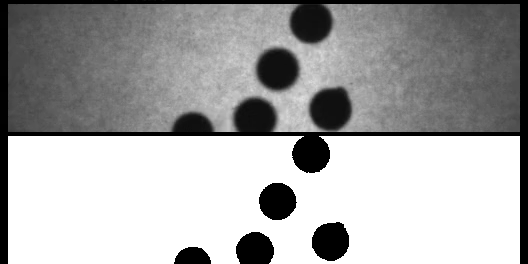
\includegraphics[clip,width=7.0cm]{bb.png}
	\caption{二値化画像の例 上:撮影された映像の1フレーム、下:二値化画像}
	\label{fig:threshold}
\end{figure}

\section{測定方法}
測定に用いるのは落下装置とハイスピードカメラである。落下装置はダンボール箱を加工したもので、光を通したり撮影したりするための穴や物体を充填する漏斗とストッパーで構成されている。装置とカメラの位置関係を図\ref{fig:equip}に示す。2つの距離は70 cmとし、カメラに映っている範囲で物体の落下速度は約2 m/sとなるようにしている。
\subsection{物体の種類}
本研究で測定した物体は表\ref{tb:ballkind}に示す7種類である。 \\
\begin{table}[H]
	\caption{実験に使用した物体 \label{tb:ballkind}}
	\begin{tabular}{lr}
		\toprule
		種類 & 直径[mm] \\
		\midrule
		金属球 & 6.2 \\
		BB弾 & 6.0 \\
		発泡ポリスチレン & 1.54 \\
		砂(15〜20メッシュ) & 1 \\
		砂(20〜30メッシュ) & 0.7 \\
		海砂(150〜200メッシュ) & 0.08 \\
		水(白絵の具で着色) & - \\
		\bottomrule
	\end{tabular}
\end{table}

表\ref{tb:ballkind}で金属球、BB弾、発泡ポリスチレンは実際に測定したものだが、砂と海砂については表記されたメッシュ値を参考におおよその直径を決めている。 \par
カメラのシャッタースピードは5000 fps($\frac{1}{5000}秒に1回$)、露光時間は$\frac{1}{80000}秒$である。 \par
本研究においてほとんどの物体は黒背景にして白色で抜き出している。これは物体にライトを当てることによって物体が白っぽく映るためであるが、金属球については反射によって色のむらができてしまうため、白背景にして後ろから光を当てることにより黒で抜き出している。
ガラスビーズの測定も試みたが、金属球と同様反射する他光を透過するため前述のように逆光で黒く抜き出すことも困難であった。

\section{各物体の評価}
\subsection{相関関数}
実験で得られた各物体の相関関数を下記にまとめる。
前述したように$相関関数G(\Delta t)$は0〜1の値をとる。
また、定義域は$\Delta t=0〜0.1秒$である。 \par
図\ref{fig:overall}は0.1秒間にどれだけ相関が減少したかを表している。
砂や水といった物質はほとんど相関が減少していないことがわかる。
これらの物体は人の目から見ても帯状の塊が連なって落ちていることがわかる。
すなわち、粒ひとつひとつが独立して動くことがなく、なだらかな動きを見せるのである。
このような場合撮影したどのフレームを見ても形は大きく変わっていないことがわかる。 \par
\begin{figure}[H]
	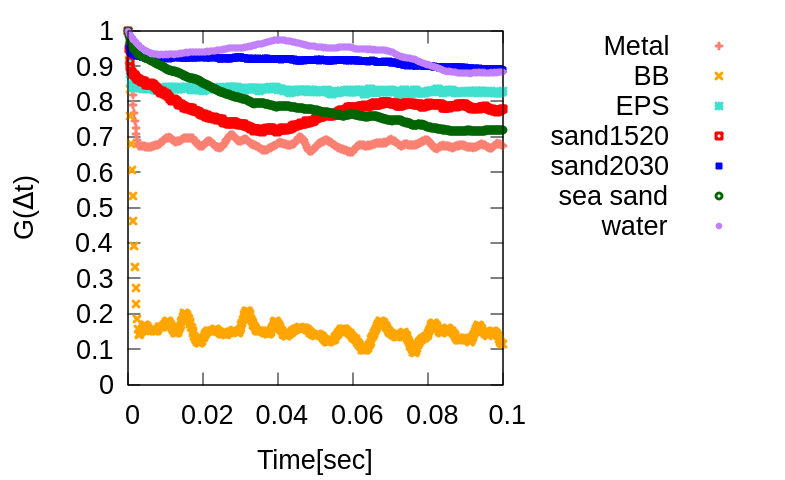
\includegraphics[scale=0.4]{overall.png}
	\caption{各物体の相関関数}
	\label{fig:overall}
\end{figure}
多くの場合において初期状態($G(0)=1$,完全一致)から急激な減少が起こっていることがわかる。
この部分を拡大したグラフが図\ref{fig:init}である。
金属球、BB弾のように直径が大きいものについては0.003秒まで減少が続いている。
砂などは0.001秒付近、水については今回プロットした間隔や範囲では相関喪失が確認できなかった。
少なくとも固体については直径が小さくなるほど相関喪失が早くなるようである。 \par
\begin{figure}[H]
	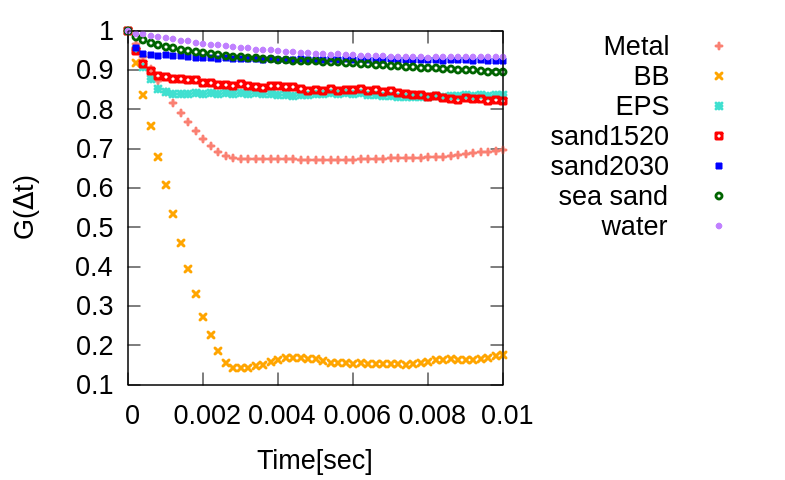
\includegraphics[scale=0.4]{init.png}
	\caption{各物体の相関関数(0.004秒まで)}
	\label{fig:init}
\end{figure}
図\ref{fig:diff}は微分を用いることによって相関減少の速度を調べたものである。
相関喪失の終わりは傾きがほぼ0になる。
傾き0となる順に物体を列挙すると次のようになる。\\
水(ただし0に限りなく近くは通るが0にはならない)、砂20-30メッシュ、砂15-20メッシュ、発泡ポリスチレン、BB弾、金属球 ※発泡ポリスチレンについては喪失点が見られなかった\\
直径と相関喪失の間には関係性があることがわかる。
この関係性を散布図に図示すると図\ref{fig:zero}となる。

\begin{figure}[H]
	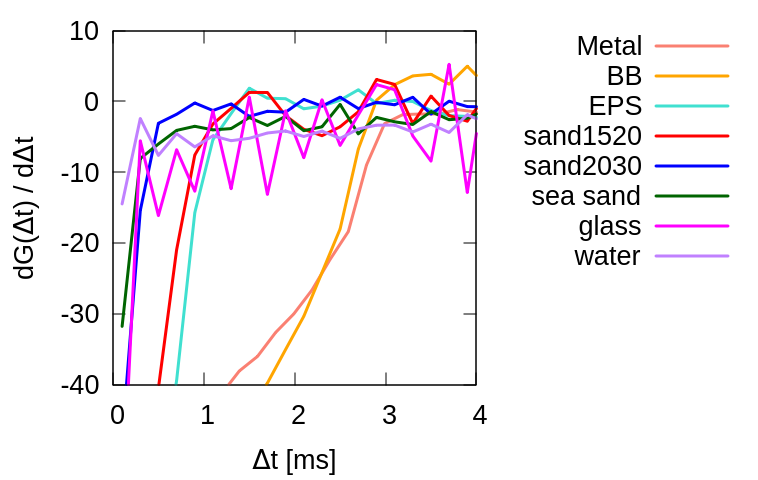
\includegraphics[scale=0.4]{diff.png}
	\caption{各物体の相関関数の微分}
	\label{fig:diff}
\end{figure}
\begin{figure}[H]
	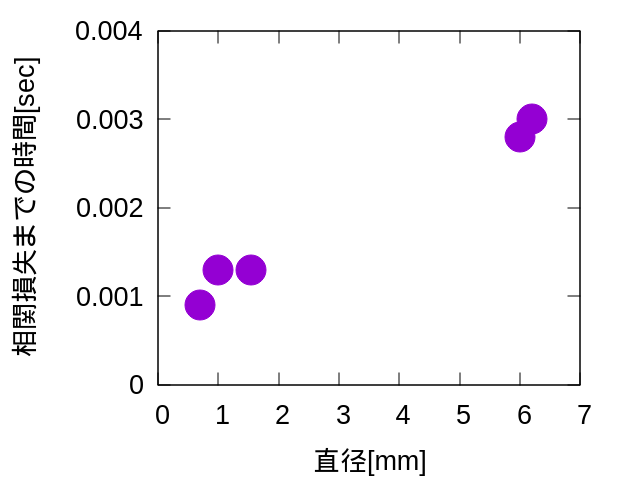
\includegraphics[scale=0.4]{zeropoint.png}
	\caption{各物体の相関関数の微分}
	\label{fig:zero}
\end{figure}

\end{document}
